% Cover
\definecolor{ccolor1}{RGB}{236,145,143}
\definecolor{ccolor2}{RGB}{131,168,192}
\definecolor{ccolor3}{RGB}{182,227,150}
\definecolor{ccolor4}{RGB}{171,206,145}

\begin{titlepage}

    \newgeometry{top=1cm, width=21cm, bottom=1cm}

    \begin{tikzpicture}[remember picture,overlay,every node/.style={anchor=center}]
        \node[opacity =0.07, inner sep=0pt, anchor=east] at (current page.east){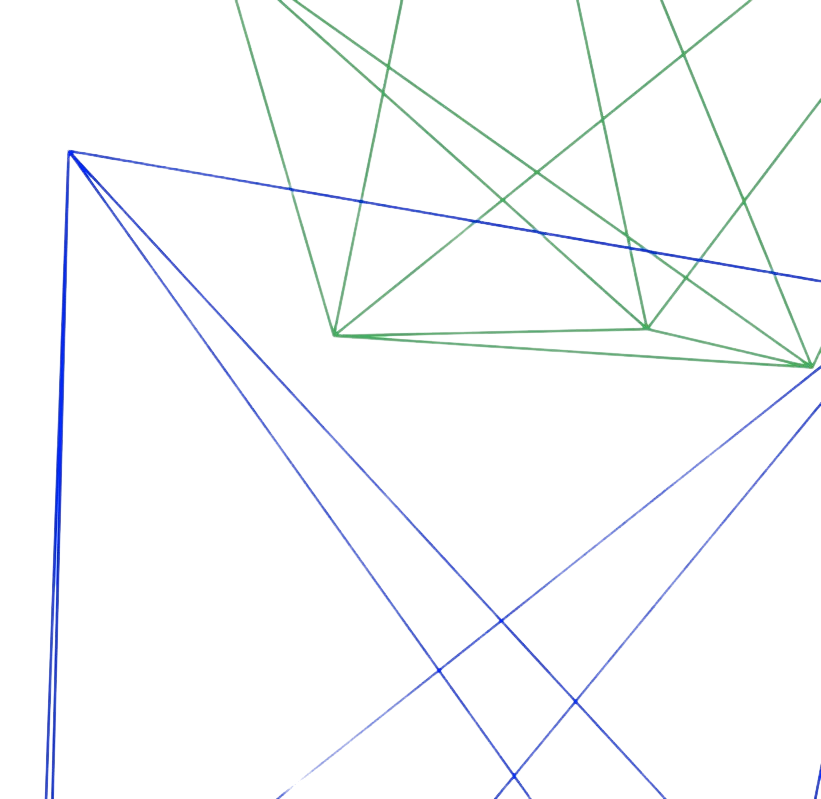
\includegraphics[width=0.5\paperwidth,height=\paperheight]{/home/archlinux/.config/latex-utils/logos/invert1.png}};

        %\node[opacity=0.15, inner sep=0pt, anchor=south west] at (current page.south west){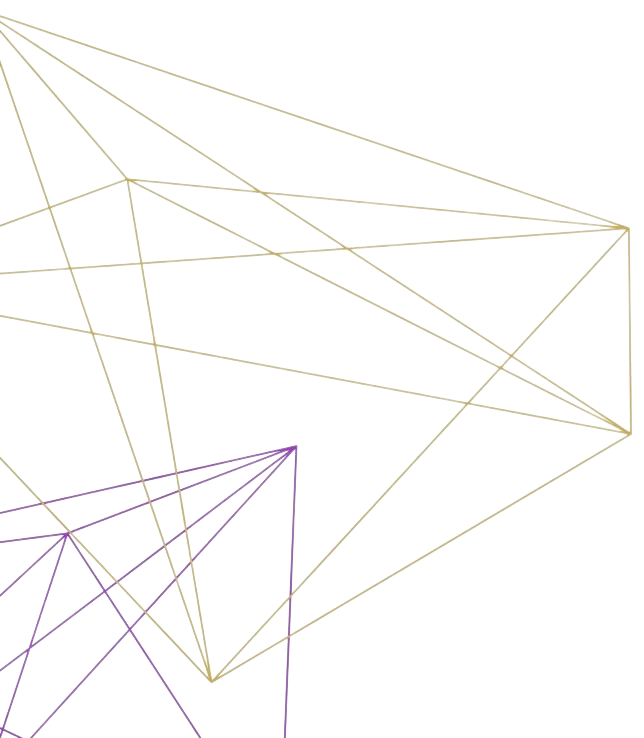
\includegraphics[width=0.5\paperwidth,height=0.5\paperheight]{/home/archlinux/.config/latex-utils/logos/invert2.png}};

        \node[opacity=0.15,inner sep=0pt, anchor=north west] at (current page.north west){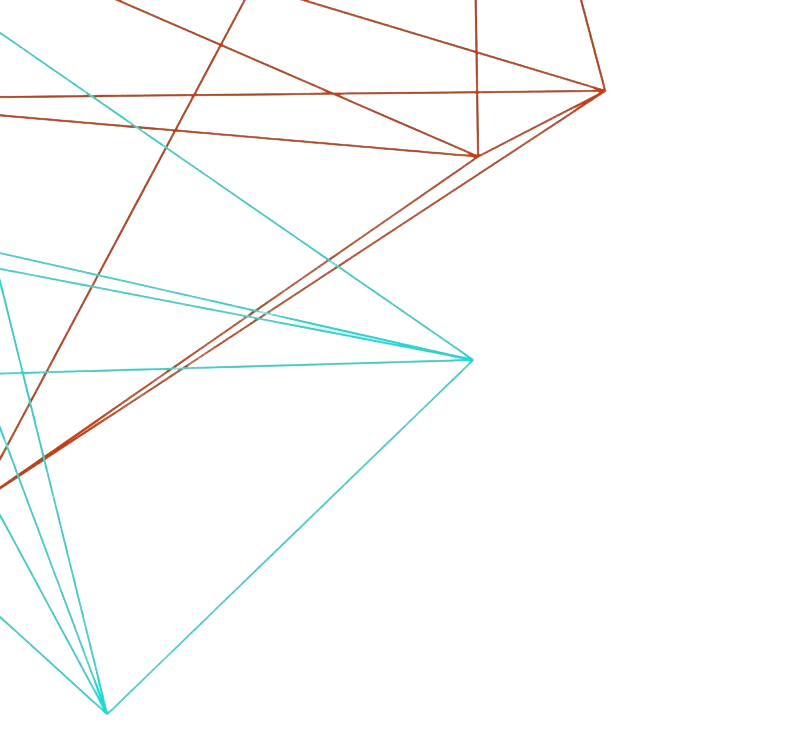
\includegraphics[width=0.5\paperwidth,height=0.5\paperheight]{/home/archlinux/.config/latex-utils/logos/invert3.png}};

        \node at (page cs:0,0.875) {\Large\bfseries\textsc{FISE 1}};
        \node at (page cs:0,0.925) {\LARGE\bfseries\textsc{Telecom Saint-Étienne}};


        %\node[opacity=0.15, inner sep=0pt, anchor=south west] at (current page.south west){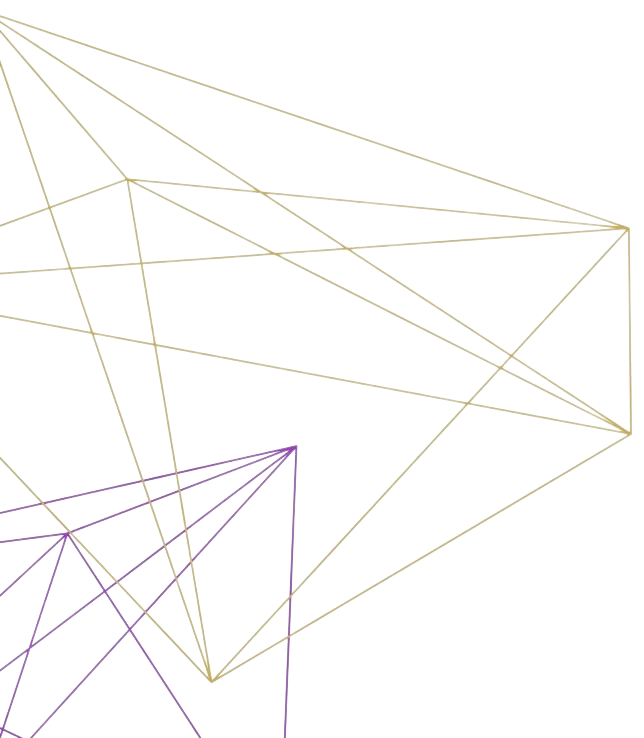
\includegraphics[width=0.5\paperwidth,height=0.5\paperheight]{/home/archlinux/.config/latex-utils/logos/invert2.png}};

        \node at (page cs:0,0.6) {\fontsize{28}{28.8}\textbf{\ctoptitle}};
        \node at (page cs:0,0.525) {\fontsize{28}{28.8}\textbf{\ctitle}};
        \draw (page cs:0.5,0.475) -- (page cs:-0.5,0.475);
        \node at (page cs:0,0.445) {\Large\textsc{Étude en Filière Ingénieur sous Statut Étudiant}};
        \node at (page cs:0,0.4) {\Large\textsc{\cdate}};
        \node at (page cs:0,0.335) {\LARGE\textsc{\cautor}};

        \node at (page cs:0,0.9) {
\includegraphics[height=2.25cm]{/home/archlinux/.config/latex-utils/logos/UJM.png}\hspace{11cm}
\includegraphics[height=1.5cm]{/home/archlinux/.config/latex-utils/logos/IMT.png}};

    \end{tikzpicture}

    % Telecom Logo Big
    \begin{tikzpicture}[remember picture,overlay,every node/.style={anchor=south west}]
        \fill[thin, fill=ccolor1, opacity=1] (page cs: -1,-0.39) arc (124.5:-4.7:10cm) -- (page cs: -1,-1) -- (page cs: -1,-0.39);
        \fill[thin, fill=ccolor2, opacity=1] (page cs: -1,-0.14) arc (92.3:53.25:10cm) arc (85.9:124.5:10cm) -- (page cs: -1,-0.14);
        \fill[thin, fill=ccolor3, opacity=1] (page cs: -1,-0.005) arc (106:18.7:10cm) arc(49:85.9:10cm) arc (53.25:92.3:10cm) -- (page cs: -1,-0.005);
        \fill[thin, fill=ccolor4, opacity=1] (page cs: -0.06,-1) arc (-16.65:52.5:10cm) arc (85.9:49:10cm) arc (18.7:-34:10cm) -- (page cs: -0.06,-1);
        \fill[thin, fill=white, opacity=1] (page cs: -0.17,-1) -- (page cs: -0.17,-0.523) -- (page cs: -0.525,-0.374) -- (page cs: -1,-0.57) -- (page cs: -1,-1) -- (page cs: -0.925,-1) -- (page cs: -0.925,-0.833) -- (page cs: -0.515,-0.665) -- (page cs: -0.515,-1) -- (page cs: -0.17,-1);
    \end{tikzpicture}
\end{titlepage}

\newgeometry{left=2.5cm, width=16cm, bottom=2.5cm, top=2.5cm}
\thispagestyle{plain}
\textcolor{white}{Blank page}


\newpage
\thispagestyle{plain}
\vspace*{\fill}

\hspace{\fill}\text{\huge\bfseries\textsc{\sectittle}}\hspace{\fill}

\hspace{\fill}\text{\huge\bfseries\textsc{\sectoptittle}}\hspace{\fill}
\vspace*{\fill}
\vspace*{\fill}
\vspace*{\fill}


\newgeometry{left=2.5cm, width=16cm, bottom=2cm, top=2cm}

\tikz[remember picture, overlay] \node[opacity=0.15,inner sep=0pt, anchor=north east] at (current page.north east){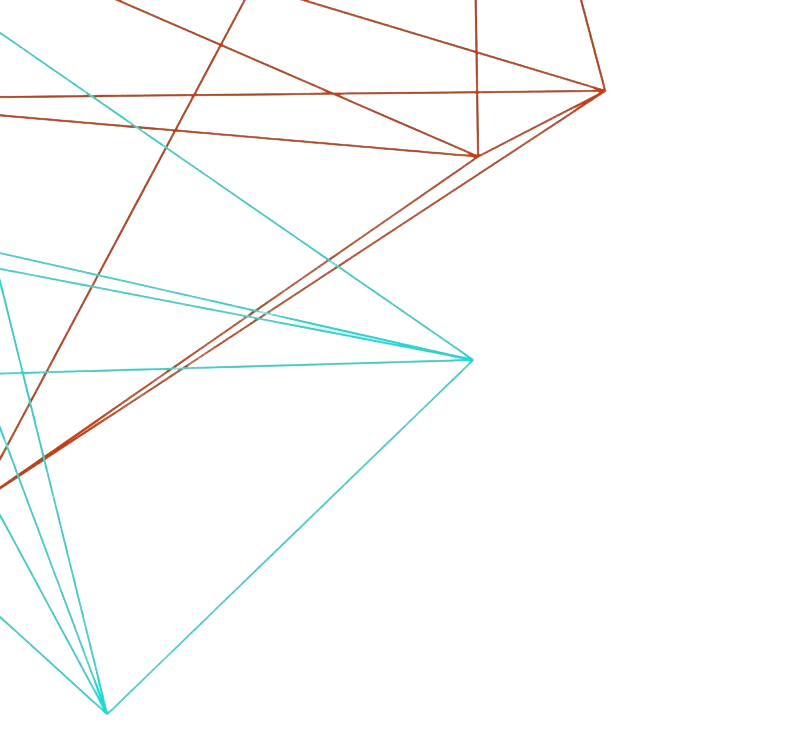
\includegraphics[angle=-90,origin=c,width=0.5\paperheight,height=0.5\paperwidth]{/home/archlinux/.config/latex-utils/logos/invert3.png}};
\tikz[remember picture,overlay] \node[opacity=0.15,inner sep=0pt, anchor=south east] at (current page.south east){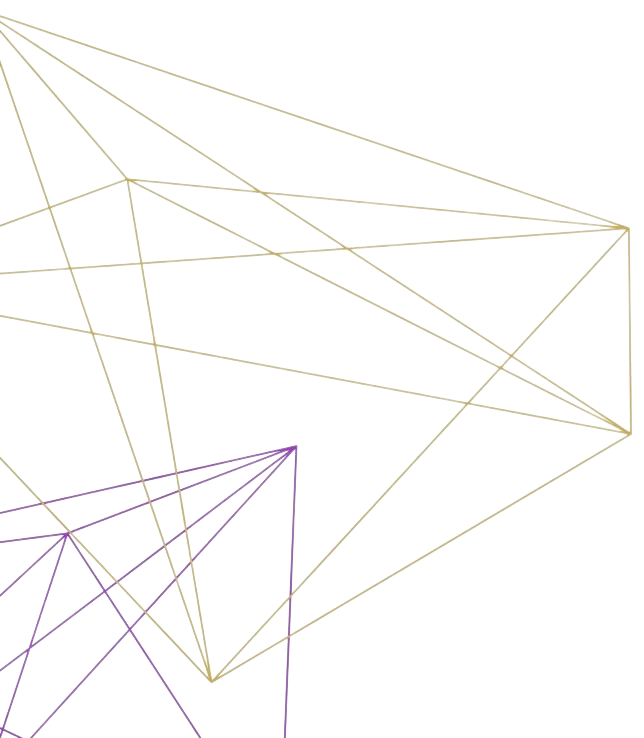
\includegraphics[angle=90,width=0.5\paperwidth,height=0.5\paperheight]{/home/archlinux/.config/latex-utils/logos/invert2.png}};

\tableofcontents

\newgeometry{left=2.5cm, width=16cm, bottom=2.5cm, top=2.5cm}

